\subsubsection{XL6009}

El regulador conmutado elevador (o Boost converter en inglés) es un módulo que permite elevar una tensión de entrada más baja a una tensión de salida mayor. Esto se logra pidiendo más corriente a la entrada y entregando menos corriente a la salida.\cite{xlsemi400KHz604}

En este caso, se utiliza para elevar la tensión de la batería de backup (tensión de $12 V$) a una tensión de $24 V$ para alimentar el sistema.

\begin{figure}[h]
    \centering
    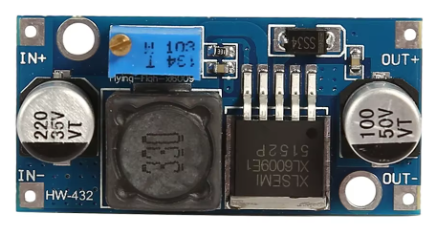
\includegraphics[width=0.5\textwidth]{images/2-hardware/componentes/XL6009.png}
    \caption{Módulo regulador elevador \texttt{XL6009}}
    \label{fig:hardware/modulos/xl6009}
\end{figure}